\documentclass[journal,12pt,twocolumn]{IEEEtran}

\usepackage{enumitem}
\usepackage{amsmath}
\usepackage{amssymb}
\usepackage{gensymb}
\usepackage{graphicx}
\usepackage{txfonts}         
\usepackage{listings}
\usepackage{lstautogobble}
\usepackage{mathtools}

\newcommand{\solution}{\noindent \textbf{Solution: }}
\providecommand{\pr}[1]{\ensuremath{\Pr\left(#1\right)}}
\providecommand{\brak}[1]{\ensuremath{\left(#1\right)}}
\providecommand{\cbrak}[1]{\ensuremath{\left\{#1\right\}}}
\providecommand{\sbrak}[1]{\ensuremath{\left[#1\right]}}
\providecommand{\mean}[1]{E\left[ #1 \right]}
\providecommand{\var}[1]{\mathrm{Var}\left[ #1 \right]}
\providecommand{\der}[1]{\mathrm{d} #1}

\let\StandardTheFigure\thefigure
\numberwithin{equation}{section}
\renewcommand{\thefigure}{\theenumi}
\renewcommand\thesection{\arabic{section}}

\lstset {
	frame=single, 
	breaklines=true,
	columns=fullflexible,
	autogobble=true
}             
\title{Random Numbers \\ \Large AI1110}
\author{I Sai Pradeep \\ \normalsize AI21BTECH11013 \\ \vspace*{20pt} \normalsize  \today}

\begin{document} 


	\maketitle
	\tableofcontents

	\section{Uniform Random Numbers}
	Let $U$ be a uniform random variable between 0 and 1.
	\begin{enumerate}[label=\thesection.\arabic*,ref=\thesection.\theenumi]
	\item Generate $10^6$ samples of $U$ using a C program and save into a file called uni.dat

	\solution Download the C source code by executing the following commands
	\begin{lstlisting}
wget https://github.com/Pradeep8802/Random_numbers/blob/main/1.1/exrand.c
wget https://github.com/Pradeep8802/Random_numbers/blob/main/1.1/coeffs.h
            
	\end{lstlisting}
	Compile and run the C program by executing the following
	\begin{lstlisting}
cc exrand.c -lm
./a.out
        \end{lstlisting}
	\item Load the uni.dat file into Python and plot the empirical CDF of $U$ using the samples in uni.dat. The CDF is defined as
	\begin{align}
		F_{U}(x) = \pr{U \le x}
	\end{align}

	\solution  The following code plots Fig. \ref{fig-1.2}
	\begin{lstlisting}
wget https://github.com/Pradeep8802/Random_numbers/tree/main/1.2/cdf_U.py
        \end{lstlisting}
	Run the code by executing the below command  
	\begin{lstlisting}
python3 cdf_U.py
	\end{lstlisting}
	\begin{figure}
		\centering
		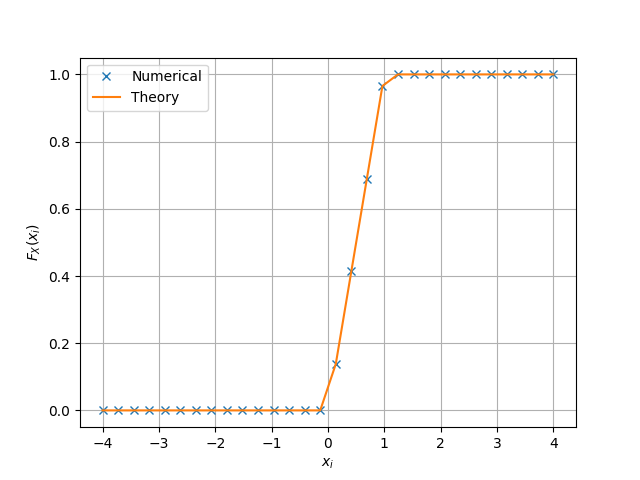
\includegraphics[width=\columnwidth]{../figs/cdf_1.2.png}
		\caption{The CDF of $U$}
		\label{fig-1.2}
	\end{figure}
	\item Find a  theoretical expression for $F_{U}(x)$
	
	\solution Here $U$ is a uniform random variable in $[0,1]$. The PDF of $U$ is given as follows
 
	\begin{align}
		p_{U}(x) = 
		\begin{cases}
			1 & x \in [0, 1] \\
			0 & \text{otherwise}
		\end{cases}
	\end{align}
        The CDF of $U$ is 
        \begin{align}
		F_{U}(x) = \pr{U \le x} 
	\end{align}
        Since, 
        \begin{align}
		\pr{U \le x}=\int_{-\infty}^x p_{U}(x) ~\mathrm{d}x 
	\end{align}
     %   $\therefore$ 
	\begin{align*}
    \therefore F_{U}(x) = \int_{-\infty}^x p_{U}(x) ~\mathrm{d}x
	\end{align*}
	If $x<0$,
	\begin{align}
\int_{-\infty}^x p_{U}(x) ~\mathrm{d}x &= \int_{-\infty}^x 0 ~\mathrm{d}x \\
&= 0\\
F_{U}(x)=0
	\end{align}
	If  $ 0 \leq x \leq 1 $,
	\begin{align}
		\int_{-\infty}^x p_{U}(x) ~\mathrm{d}x &= \int_{-\infty}^0 0 ~\mathrm{d}x + \int_0^x 1 ~\mathrm{d}x \\
		&= 0 + x \\
		&= x\\
            F_{U}(x)=x
	\end{align}
	If $x>1$,
	\begin{multline}
		\int_{-\infty}^x p_{U}(x) ~\mathrm{d}x \\= \int_{-\infty}^0 0 ~\mathrm{d}x + \int_0^1 1 ~\mathrm{d}x +  \int_1^x 0 ~\mathrm{d}x 
	\end{multline}
	\begin{align}
		\int_{-\infty}^x p_{U}(x) ~\mathrm{d}x &= 0 + 1 + 0 \\
		&= 1\\
            F_{U}(x)=1
	\end{align}
	Hence the CDF of $U$ is 
	\begin{align}
		F_{U}(x) = 
		\begin{cases}
			0 & x < 0 \\
			x & 0 \le x \le 1 \\
			1 & x > 1
		\end{cases}
	\end{align}
	
	\item The mean of $U$ is defined as
	\begin{align}
		\mean{U} = \frac{1}{N}\sum_{i=1}^{N}U_i
	\end{align}
	and its variance as
	\begin{align}
		\var{U} = E[(U-E[U])^2]
	\end{align}
	Write a C program to  find the mean and variance of $U$
	
	\solution Download the following codes and execute the C program
	\begin{lstlisting}
wget https://github.com/Pradeep8802/Random_numbers/blob/main/1.4/mean_variance.c
wget https://github.com/Pradeep8802/Random_numbers/blob/main/1.1/coeffs.h
	\end{lstlisting}
Run the code by executing the below command
\begin{lstlisting}
cc mean_variance.c -lm
./a.out
\end{lstlisting}
	The output of the code is
	\begin{align}
		\mu &= 0.500007 \\
		\sigma^2 &= 0.083301 
	\end{align}
	
	\item Verify your result theoretically given that
	\begin{align}
		\mean{U^k} = \int_{-\infty}^{\infty}x^k \mathrm{d}F_{U}(x)
	\end{align}
		
	\solution The mean of $U$ is given by
	%\begin{align}
	%	\mean{U} = \int_{-\infty}^{\infty}x ~\mathrm{d}F_{U}(x) 
	%\end{align}
        \begin{align}
		\mean{U} = \int_{-\infty}^{\infty}x ~\mathrm{d}x 
	\end{align}
        The CDF of $U$ is
        \begin{align}
		F_{U}(x) = 
		\begin{cases}
			0 & x < 0 \\
			x & 0 \le x \le 1 \\
			1 & x > 1
		\end{cases}
	\end{align}
 On differentiating the above CDF, we have
	\begin{align}
		\mathrm{d}F_{U}(x) = 
		\begin{cases}
			\mathrm{d}(0) & x < 0 \\
			\mathrm{d}(x) & 0 \le x \le 1 \\
			 \mathrm{d}(1) & x > 1
		\end{cases}
	\end{align}

 \begin{align}
		\mathrm{d}F_{U}(x) = 
		\begin{cases}
			0 & x < 0 \\
			\mathrm{d}x & 0 \le x \le 1 \\
			0 & x > 1
		\end{cases}
	\end{align}

\begin{align}
\mean{U} = \int_{-\infty}^{\infty}x ~\mathrm{d}F_{U}(x) 
\end{align}
 \begin{align}    
E[U^k]=\int_{-\infty}^{\infty} x^k \mathrm{d}(x)\\
E[U]=\int_{0}^{1} x \mathrm{d}(x)=\frac{1}{2}\\
E[U^2]=\int_{0}^{1} x^2 \mathrm{d}x
&=\frac{1}{3}\\
Var(U)=E[U^2]-(E[U])^2=\frac{1}{12}
 \end{align}
Hence,
\begin{align}
		E[U]=\frac{1}{3} \approx 0.5\\
            \mu = 0.5\\
            Var(U) = \frac{1}{12} \approx 0.083333\\
            \sigma=0.083333\\
            \Delta \mu \approx 0.000007\\
            \Delta \sigma \approx 0.000032 
	\end{align}

	\section{Central Limit Theorem}

	\begin{enumerate}[label=\thesection.\arabic*,ref=\thesection.\theenumi]
	\item Generate $10^6$ samples of the random variable
	\begin{align}
		X = \sum_{i=1}^{12}U_i -6
	\end{align}

	using a C program, where $U_i, i = 1,2,\dots, 12$ are  a set of independent uniform random variables between 0 and 1 and save in a file called gau.dat
	
	\solution Download the following codes and execute the C program
	\begin{lstlisting}
wget https://github.com/Pradeep8802/Random_numbers/blob/main/2.1/2.1.c
wget https://github.com/Pradeep8802/Random_numbers/blob/main/2.1/coeffs.h
	\end{lstlisting}
	 Run the code by executing the below command
	\begin{lstlisting}
cc 2.1.c -lm
./a.out
	\end{lstlisting}
		
	\item Load gau.dat in Python and plot the empirical CDF of $X$ using the samples in gau.dat. What properties does a CDF have?

	\solution Download the following code and execute the Python program
	\begin{lstlisting}
wget https://github.com/Pradeep8802/Random_numbers/blob/main/2.2/cdf_gaussian.py
	\end{lstlisting}
	Run the code by executing the below command
	\begin{lstlisting}
python3 cdf_gaussian.py
	\end{lstlisting}
	\begin{figure}
		\centering
		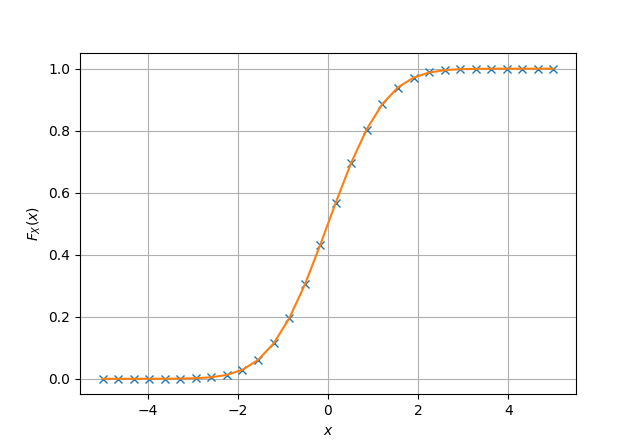
\includegraphics[width=\columnwidth]{../figs/cdf_gaussian.png}
		\caption{The CDF of $X$}
		\label{fig-2.2}
	\end{figure}


Properties of CDF:
\begin{enumerate}[label=(\alph*)]
\item It is always continuous.
\item It always lies in [0,1]
\item Q function is defined as:
	\begin{align}
		Q_X(x)=\pr{x<X}\\
	\therefore F_X\brak{x}=1-Q_X\brak{x}
	\end{align}
\item CDF $(F_{X}(x))$ is non-decreasing function as it is the sum of non-negative probabilities.
\end{enumerate}

	\item Load gau.dat in Python and plot the empirical PDF of $X$ using the samples in gau.dat. The PDF of $X$ is defined as
	\begin{align}
		p_{X}(x) = \frac{d}{dx}F_{X}(x)
	\end{align}
	What properties does the PDF have?
	
	\solution Download the following code and execute the Python program
	\begin{lstlisting}
wget https://github.com/Pradeep8802/Random_numbers/blob/main/2.3/pdf_gaussian.py
	\end{lstlisting}
	Run the code by executing the below command
	\begin{lstlisting}
python3 pdf_gaussian.py
	\end{lstlisting}
	\begin{figure}
		\centering
		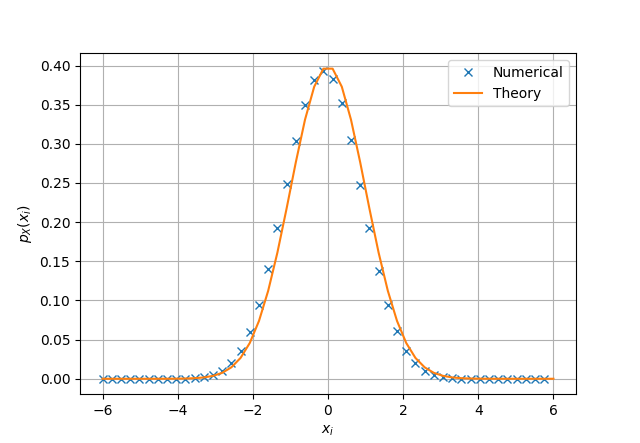
\includegraphics[width=\columnwidth]{../figs/pdf_gaussian.png}
		\caption{The PDF of $X$}
		\label{fig-2.3}
	\end{figure}

Properties of PDF:
\begin{enumerate}[label=(\alph*)]
    
\item PDF$(p_{X}(x))$ is bounded between [0,1]
\item PDF is a bell-shaped curve
\item PDF graph has symmetry around the mean of the distribution
\item If $\mu$ is the mean of the distribution,  here $p_{X}(x)$ is symmetric with respect to 0, since here $\mu=0$ $(\mathcal{N}(0,1))$
\end{enumerate}
	\item Find the mean and variance of $X$ by writing a C program
	
	\solution Download the following code and execute the C program
	\begin{lstlisting}
wget https://github.com/Pradeep8802/Random_numbers/blob/main/2.4/coeffs.h
wget https://github.com/Pradeep8802/Random_numbers/blob/main/2.4/mean_variance_gaussian.c
	\end{lstlisting}
	Run the code by executing the below command
\begin{lstlisting}
cc mean_variance_gaussian.c -lm
./a.out
\end{lstlisting}
	\begin{align}
            \mu &= 0.000326\\
            \sigma &= 1.000906\\
		\text{Mean} &= 0.000326 \\
		\text{Variance} &= 1.000906 
	\end{align}	
 
	\item Given that
	\begin{align}
		p_{X}(x) = \frac{1}{\sqrt{2\pi}}\exp\brak{-\frac{x^2}{2}}, -\infty < x < \infty,
	\end{align}
	repeat the above exercise theoretically
	
	\solution 
        As $p_{X}(x)$ is given,
        Hence, the mean of $X$ is 
	\begin{align}
		&\mean{X} = \int_{-\infty}^{\infty} \frac{x}{\sqrt{2\pi}}\exp\brak{-\frac{x^2}{2}} \mathrm{d}x \\
  		&\mean{X} = \frac{1}{\sqrt{2\pi}} \int_{-\infty}^{\infty} x \exp\brak{-\frac{x^2}{2}} \mathrm{d}x   \\
&=\frac{1}{\sqrt{2\pi}} \int_{-\infty}^{0} x \exp\brak{-\frac{x^2}{2}} \mathrm{d}x \nonumber \\ 
&+\frac{1}{\sqrt{2\pi}} \int_{0}^{\infty} x \exp\brak{-\frac{x^2}{2}} \mathrm{d}x 
        \end{align}

Let $g(x)=x e^{-\frac{-x^2}{2}} $

Consider $\int_{-\infty}^{0} g(x) \mathrm{d}x$

Substituting z=-x, we get
\begin{align}
\int_{-\infty}^{0} g(x) \mathrm{d}x &= \int_{\infty}^{0} g(-x) \mathrm{d}(-x) \\
&=- \int_{\infty}^{0} g(-x) \mathrm{d}(x) \\
&= \int_{0}^{\infty} g(-x) \mathrm{d}(x) \\
g(-x)&= -x e^{-\frac{-(-x)^2}{2}}  \\
g(-x)&= -(x e^{-\frac{-(x)^2}{2}}) \\
g(-x)&=g(x) \\
\int_{-\infty}^{0} g(x) \mathrm{d}x &= - \int_{0}^{\infty} g(x) \mathrm{d}(x) \\
&= \frac{1}{\sqrt{2\pi}} \int_{-\infty}^{\infty} x \exp\brak{-\frac{x^2}{2}} \mathrm{d}x \\
&=\int_{0}^{\infty} g(x) \mathrm{d}(x)- \int_{0}^{\infty} g(x) \mathrm{d}(x) = 0 
\end{align}
$\therefore$ Mean = 0

Let
\begin{align}
h(x)&=\frac{x^2}{\sqrt{2\pi}}\exp\brak{-\frac{x^2}{2}} \\
h(-x)&=\frac{(-x)^2}{\sqrt{2\pi}}\exp\brak{-\frac{(-x)^2}{2}} \\
&=\frac{x^2}{\sqrt{2\pi}}\exp\brak{-\frac{x^2}{2}} \\
\end{align}
$\therefore h(-x)=h(x)$
\begin{align}
\therefore \int_{-\infty}^{0} \frac{x^2}{\sqrt{2\pi}}\exp\brak{-\frac{x^2}{2}} \mathrm{d}x=\int_{0}^{\infty} \frac{x^2}{\sqrt{2\pi}}\exp\brak{-\frac{x^2}{2}} \mathrm{d}x
\end{align}
\begin{align}
 \mean{X^2} &= \int_{-\infty}^{\infty} \frac{x^2}{\sqrt{2\pi}}\exp\brak{-\frac{x^2}{2}} \mathrm{d}x \\
&= 2 \int_{0}^{\infty} \frac{x^2}{\sqrt{2\pi}}\exp\brak{-\frac{x^2}{2}} \mathrm{d}x
	\end{align}
	Using integration by parts,
	\begin{align}
		\mean{X^2} = \sqrt{\frac{2}{\pi}}  \int_{0}^{\infty} (x) \cdot (x \exp\brak{-\frac{x^2}{2}}) dx
       \end{align}
	\begin{multline}
		= \sqrt{\frac{2}{\pi}} \brak{\left. x \int x \exp\brak{-\frac{x^2}{2}} dx}\right|_0^{\infty} \\- \sqrt{\frac{2}{\pi}}  \int_{0}^{\infty} 1 \cdot (\int x \exp\brak{-\frac{x^2}{2}})dx
	\end{multline}
	\begin{align}
     \text{Substituting} \hspace{3mm} z = \frac{x^2}{2} \implies dz = xdx\nonumber \\
      \end{align}
      \begin{align}
		&\int x \exp\brak{-\frac{x^2}{2}} dx = \int \exp(-z) dz \\
		&= - \exp(-z)  \\
		&= - \exp\brak{-\frac{x^2}{2}} 
\end{align}
Substituting $x = \sqrt{2} t$ 
\begin{align}
\int_0^{\infty} \exp(-t^2) \sqrt{2} dt &= {\sqrt{2}}
\int_0^{\infty} \exp(-t^2) dt \\
		&=\sqrt{\frac{\pi}{2}}\\
E[X^2] &= 0 - \sqrt{\frac{2}{\pi}} \brak{- \sqrt{\frac{\pi}{2}}} \\
		&= 1 \\
\therefore Var[X] &= \mean{X^2} - \brak{\mean{X}}^2 \\
		&= 1 - 0  \\
            &= 1\\
Var[X]=1
\end{align}
	\end{enumerate}

	\section{From Uniform to Other}
	\begin{enumerate}[label=\thesection.\arabic*,ref=\thesection.\theenumi]
	\item Generate samples of 
	\begin{align}
		V = -2\ln\brak{1-U}
	\end{align}
	and plot its CDF
	\end{enumerate}
	\solution Download the following code and execute the C program
	\begin{lstlisting}
wget https://github.com/Pradeep8802/Random_numbers/blob/main/3.1/3.1.c
wget https://github.com/Pradeep8802/Random_numbers/blob/main/3.1/coeffs.h
	\end{lstlisting}
	Run the code by executing the below command
	\begin{lstlisting}
cc 3.1.c -lm
./a.out
	\end{lstlisting}
	Download the following code and execute the Python program
	\begin{lstlisting}
wget https://github.com/Pradeep8802/Random_numbers/blob/main/3.1/cdf_3.1.py
	\end{lstlisting}
	Run the code by executing the below command
	\begin{lstlisting}
python3 cdf_3.1.py
	\end{lstlisting}
	\begin{figure}
		\centering
		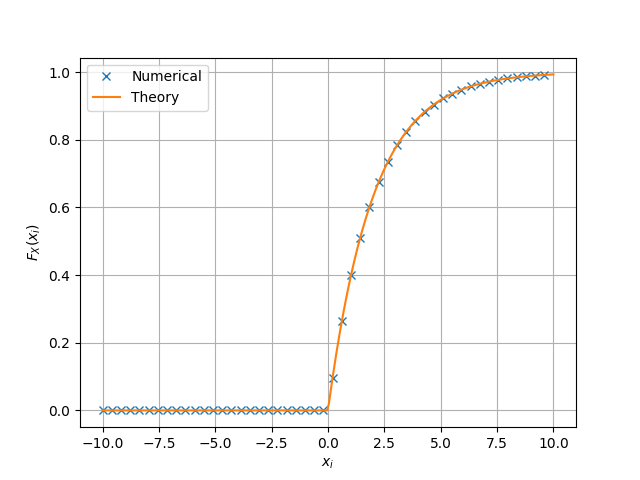
\includegraphics[width=\columnwidth]{../figs/cdf_3.1.png}
		\caption{The CDF of $V$}
		\label{fig-3.1}
	\end{figure}	
	
	\item Find a theoretical expression for $F_V(x)$	\\
	\solution 
 As $F_{V}(x)$ is the CDF of V, 
 \begin{align}
 F_{V}(x)&=P(V \leq x)\\
 &=P(-2ln(1-U) \leq x)\\
 &=-2 ln(1-U) \leq x \\
 &=ln(1-U) \geq -x/2
 \end{align}
Since ln(x) and -x/2 are monotonic, we can write
\begin{align}
 1-U \geq e^{-x/2} \nonumber
\implies 1-e^{-x/2} \leq U  \nonumber
\end{align}
 Hence,
 \begin{align}
 F_{V}(x)&=P(-2 log(1-U) \leq x)
&=P(1-e^{\frac{-x}{2}} \geq U)
\end{align}
Since,
\begin{align}
p_{U}(x) = 
		\begin{cases}
			1 & x \in [0, 1] \\
			0 & \text{otherwise}
		\end{cases} \\
 P(U<x)=\int_{0}^{x} \mathrm{d}x=x\\ 
 \therefore P(U \leq 1-e^{\frac{-x}{2}})=1-e^{\frac{-x}{2}}, \forall x\geq 0
 \nonumber
 \end{align}
 
	\section{Triangular Distribution}
	\begin{enumerate}[label=\thesection.\arabic*,ref=\thesection.\theenumi]
	\item Generate 
	\begin{align}
		T = U_1+U_2
	\end{align}
	\solution Download the following code and execute the C program\\	\\
 \begin{lstlisting}
wget https://github.com/Pradeep8802/Random_numbers/blob/main/4.1/4.1.c
wget https://github.com/Pradeep8802/Random_numbers/blob/main/4.1/coeffs.h
	\end{lstlisting}
	Run the code by executing the below command
	\begin{lstlisting}
cc 4.1.c -lm
./a.out
	\end{lstlisting}		
 
	\item Find the CDF of $T$
	
\solution Download the following code and execute the Python program
	\begin{lstlisting}
wget https://github.com/Pradeep8802/Random_numbers/blob/main/4.2/cdf_4.2_num.py
	\end{lstlisting}
	Run the code by executing the below command
	\begin{lstlisting}
python3 cdf_4.2_num.py 
./a.out
	\end{lstlisting}		
 \begin{figure}
		\centering
		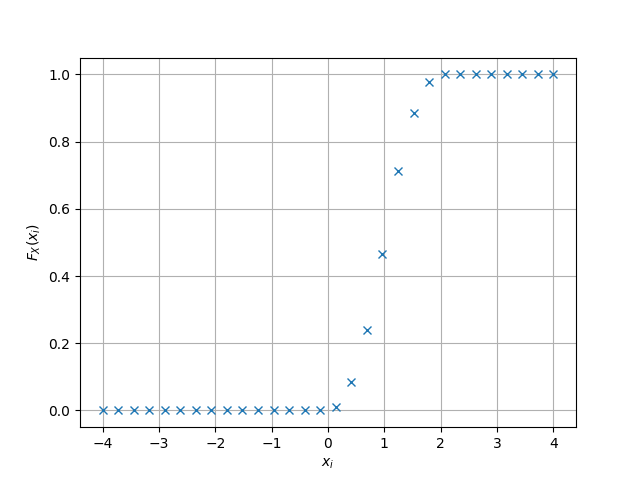
\includegraphics[width=\columnwidth]{../figs/cdf_4.2_num.png}
		\caption{The Numerical CDF of $T$}
	\end{figure}
 
 \begin{align}
T&=U1+U2\\
p_T(x) &= p_{U_1 + U_2}(x) 
 \end{align}
 Consider the convolution of the two distributions,
 \begin{align}
p_T(x) &= p_{U_1 + U_2}(x) \\
&= p_{U_1}(x) * p_{U_2}(x) \der{\tau}\\
    p_T(x) &= \int_{-\infty}^{\infty}p_{U_1}(\tau)p_{U_2}(x - \tau) \der{\tau}
    \end{align}
    
\begin{align}
\text{For} \hspace{4mm}\nonumber
\tau \in (-\infty,0) \cup (1,\infty) \\  p_{U_1}(\tau) = 0
\end{align}
Hence,
\begin{align}
p_T(x) &= \int_{-\infty}^{\infty}p_{U_1}(\tau)p_{U_2}(x - \tau) \der{\tau} \\
        &=\int_0^1p_{U_2}(x - \tau) \der{\tau}
\end{align}
\begin{align}
    \displaystyle p_T(x) = \begin{cases} 
    0 & \text{$x \leq 0$} \\  
    \int_0^x 1d\tau & \text{$0 < x < 1$} \\  
    \int_{x - 1}^1 1d\tau & \text{$1 \leq x < 2$} \\
    0 & \text{$x > 2$}
    \end{cases}
\end{align}
Hence
\begin{align}
    \displaystyle p_T(x) = \begin{cases} 
    0 & \text{$x \leq 0$} \\  
    x & \text{$0 < x < 1$} \\  
    2 - x & \text{$1 \leq x < 2$} \\
    0 & \text{$x > 2$}
    \end{cases}
\end{align}
Expression for CDF can be obtained by Integrating $p_T(x)$ w.r.t. $x$ 
\begin{align}
    \displaystyle F_T(x) = \begin{cases} 
    0 & \text{$x \leq 0$} \\  
    \frac{x^2}{2} & \text{$0 < x < 1$} \\  
    -\frac{x^2}{2} + 2x - 1 & \text{$1 \leq x < 2$} \\
    1 & \text{$x > 2$}
    \end{cases}
\end{align}
	
	\item Find the PDF of $T$
	
\solution Download the following code and execute the Python program

\begin{lstlisting}
wget https://github.com/Pradeep8802/Random_numbers/blob/main/4.3/pdf_4.3_num.py
	\end{lstlisting}
	Run the code by executing the below command
	\begin{lstlisting}
python3 pdf_4.3_num.py 
./a.out
	\end{lstlisting}	 
 The PDF of $T$ is given by
 \begin{figure}
		\centering
		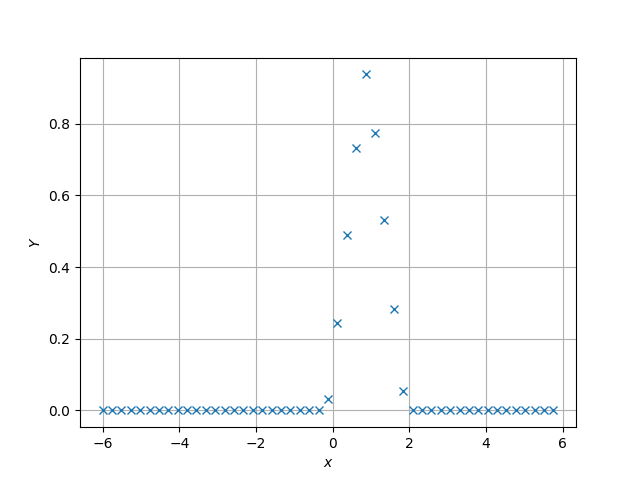
\includegraphics[width=\columnwidth]{../figs/pdf_4.3_num.png}
		\caption{The Numerical PDF of $T$}
	\end{figure}
	\begin{align}
		p_T(t) &= \frac{d(F_{T}(t))}{dt} \\
		\therefore p_T(t) &=
		\begin{cases}
			0 & t < 0 \\
			t & 0 \le t \le 1 \\
			2 - t & 1 < t < 2 \\
			0 & t \ge 2
		\end{cases}
	\end{align}
	
	\item Find the theoretical expressions for the PDF and CDF of $T$
	
	\solution 
\begin{align}
P_{T}(t)=
\begin{cases}
0 & t<0\\
t & 0\leq t \leq 1\\
2-t  & 0< t \leq 2\\
0 & t>2 
\end{cases} 
\\   
F_{T}(t)=
\begin{cases}
0 & t<0\\
\frac{t^2}{2} & 0\leq t \leq 1\\
2t -\dfrac{t^2}{2} - 1  & 1< t \leq 2\\
1 & t>2
\end{cases}
\end{align}
	\item Verify your results through a plot
	
	\solution Download the following code and execute the Python programs
	\begin{lstlisting}
wget https://github.com/Pradeep8802/Random_numbers/blob/main/4.4/cdf_4.2.py
wget https://github.com/Pradeep8802/Random_numbers/blob/main/4.4/pdf_4.3.py
	\end{lstlisting}
	Run the codes by executing the below commands for cdf and pdf respectively
	\begin{lstlisting}
python3 cdf_4.2.py
python3 pdf_4.3.py
	\end{lstlisting}
	
	
	\end{enumerate}
	
	\begin{figure}
		\centering
		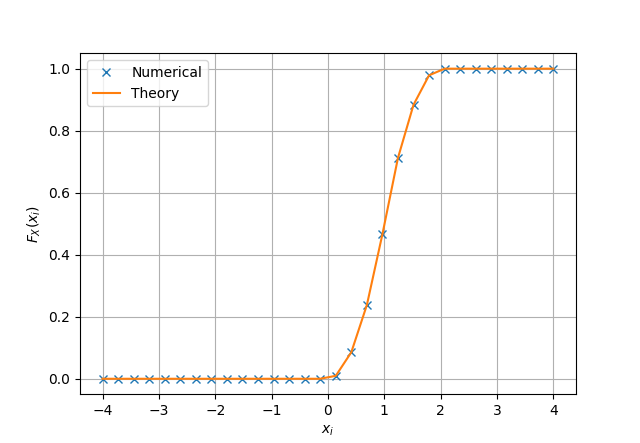
\includegraphics[width=\columnwidth]{../figs/cdf_4.2.png}
		\caption{The CDF of $T$}
	\end{figure}
	
	\begin{figure}
		\centering
		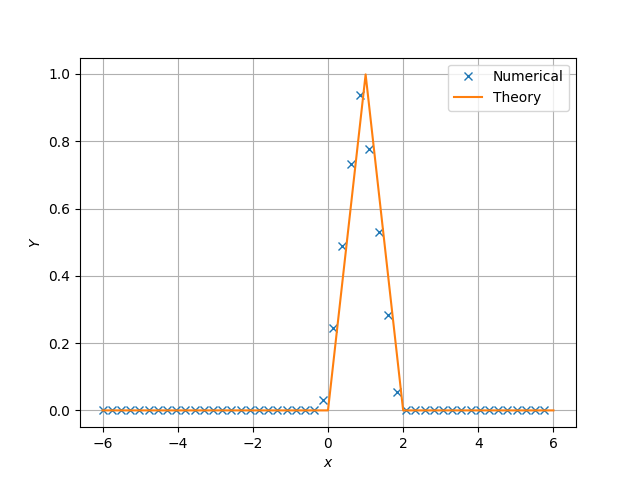
\includegraphics[width=\columnwidth]{../figs/pdf_4.3.png}
		\caption{The PDF of $T$}
	\end{figure}		
	
\end{enumerate}
\end{document}
